\chapter{Du principe d’équivalence aux tenseurs}

La relativité générale est souvent abrégée en RG, tandis que la relativité restreinte est rarement appelée RR. L’abréviation importe moins que le choix de repartir du début. Le chemin le plus direct est celui qu’a suivi Einstein : partir d’une observation physique assez simple pour être ressentie dans un ascenseur, en tirer toutes les conséquences jusqu’à ce qu’elles s’imposent, et n’introduire la géométrie qu’ensuite.

La première observation est le principe d’équivalence : la gravitation et l’accélération sont localement indiscernables. Le mot « localement » finira par porter presque tout le poids de cette affirmation. Mais avant de la nuancer, voyons ce que permet déjà d’établir l’énoncé sans réserve.

\section{L’ascenseur comme transformation de coordonnées}

Les manuels remplacent souvent l’ascenseur d’Einstein par un vaisseau spatial. L’ascenseur convient mieux ici, car son accélération nous est familière. Soit \(z\) la hauteur dans un référentiel lié au sol, et \(z'\) la hauteur mesurée depuis le plancher de l’ascenseur. Si le plancher se trouve à la hauteur \(L(t)\), un même événement a pour coordonnées
\begin{equation}
 z'=z-L(t),\qquad t'=t,\qquad x'=x.
\label{eq:elevator-map}
\end{equation}
La coordonnée horizontale ne change pas, car l’ascenseur ne glisse pas latéralement. En posant délibérément \(t'=t\), nous mettons pour l’instant la relativité restreinte de côté.

\begin{classroomqa}
\audiencequestion{Comment un cours de relativité générale peut-il commencer en ignorant la relativité restreinte ?}
\lecturerresponse{Il existe un régime où la gravitation joue un rôle alors que toutes les vitesses restent faibles devant \(c\). On peut donc isoler le lien entre la gravitation--et l’accélération en mécanique newtonienne, puis le combiner à la géométrie de Minkowski. C’est un choix de mise en place, et non l’affirmation que la théorie finale est non relativiste. \lecturetimestamp{00:05:33}}
\end{classroomqa}

Dans deux référentiels inertiels, l’ascenseur est en mouvement uniforme,
\begin{equation}
 L(t)=vt,\qquad z'=z-vt.
\label{eq:galilean-elevator}
\end{equation}
Les origines sont choisies de sorte qu’elles coïncident à \(t=0\). Le tableau garde le schéma de l’ascenseur à côté des trois relations de coordonnées, afin que les symboles conservent toujours leur sens physique.

\begin{figure}[H]
\centering
\includegraphics[width=\linewidth]{lecture_01_figure_01.png}
\caption{Coordonnées de l’ascenseur après spécialisation au cas d’une vitesse uniforme \(L(t)=vt\).}
\par\smallskip
\textit{Cadre du cours : 00:09:10.}
\end{figure}

Considérons seulement la composante verticale de la loi de Newton,
\begin{equation}
 F=m\ddot z.
\label{eq:newton-unprimed}
\end{equation}
La force peut être due à une corde, à un champ électrique ou à toute autre interaction ordinaire. En dérivant deux fois \eqref{eq:galilean-elevator}, on obtient
\(\ddot z'=\ddot z\), et donc
\begin{equation}
 F=m\ddot z'.
\label{eq:newton-primed-inertial}
\end{equation}
La forme de la loi reste inchangée. Ce calcul élémentaire met en évidence le contenu opératoire de l’équivalence entre référentiels inertiels : une transformation linéaire des coordonnées transforme un mouvement uniforme en un mouvement uniforme.

\begin{figure}[H]
\centering
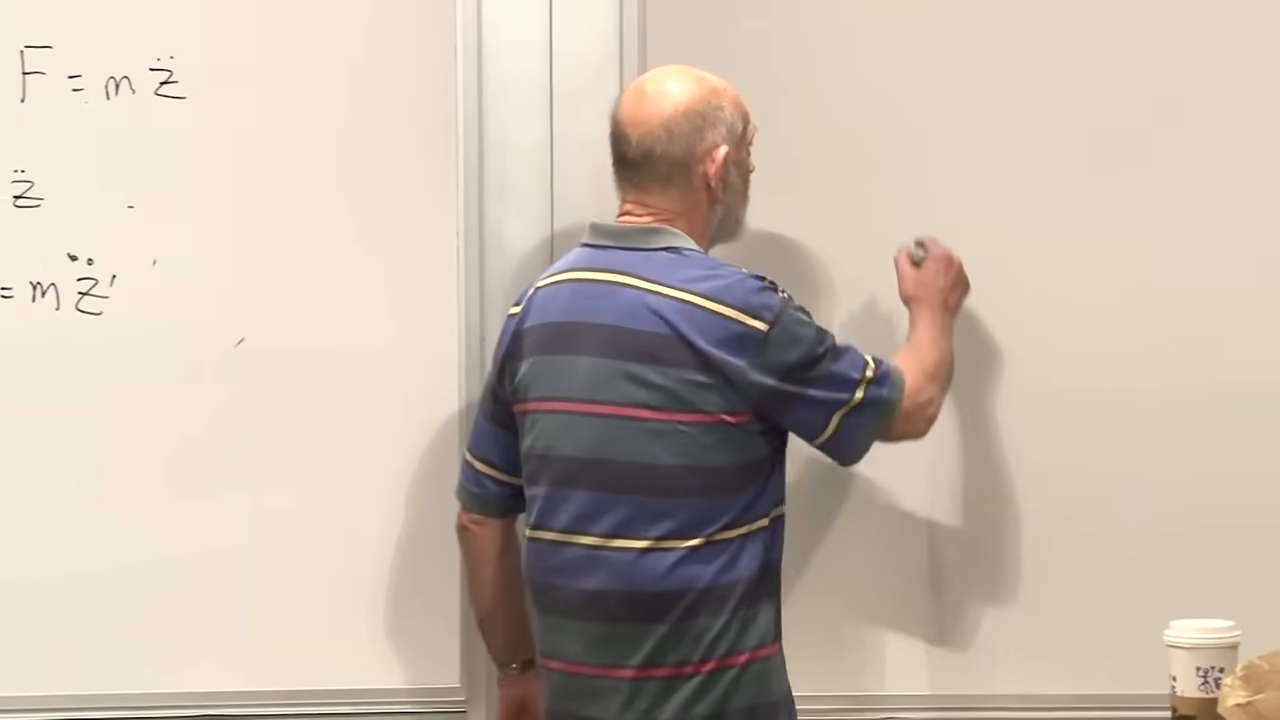
\includegraphics[width=\linewidth]{lecture_01_figure_02.png}
\caption{Équation de Newton dans deux référentiels de coordonnées en mouvement uniforme l’un par rapport à l’autre.}
\par\smallskip
\textit{Cadre du cours : 00:11:50.}
\end{figure}

Accélérons maintenant l’ascenseur vers le haut à accélération constante \(g\) :
\begin{equation}
 L(t)=\frac12gt^2,\qquad
 \dot L=gt,\qquad
 \ddot L=g.
\end{equation}
La transformation de coordonnées devient
\begin{equation}
 z'=z-\frac12gt^2,
\qquad
 \ddot z'=\ddot z-g.
\label{eq:accelerated-map}
\end{equation}
En substituant dans la loi de Newton, on obtient
\begin{equation}
 F=m(\ddot z'+g),
\qquad
 m\ddot z'=F-mg.
\label{eq:fictitious-gravity}
\end{equation}
La dérivation permet de vérifier utilement le signe en cours de route : \(+mg\) apparaît d’abord du côté de l’accélération et ne devient \(-mg\) que lorsqu’on le reporte du côté de la force. Dans le référentiel dont le plancher accélère vers le haut, le terme final est dirigé vers le bas.

\begin{figure}[H]
\centering
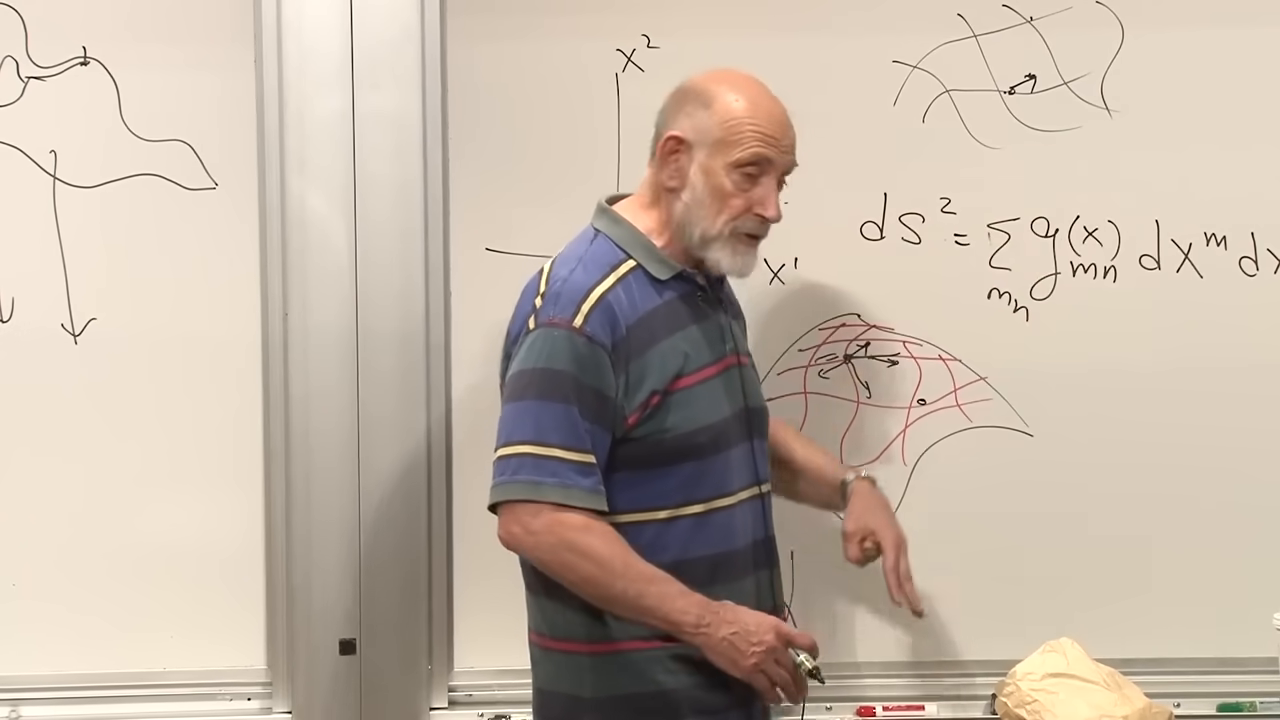
\includegraphics[width=\linewidth]{lecture_01_figure_03.png}
\caption{Transformation accélérée et force fictive qui en résulte \(-mg\).}
\par\smallskip
\textit{Cadre du cours : 00:15:35.}
\end{figure}

Le nouveau terme ressemble à la gravitation pour une raison précise : il est proportionnel à la masse. Comme la réponse inertielle est elle aussi proportionnelle à la masse, celle-ci se simplifie dans l’équation du mouvement. Un corps en chute libre suit la même trajectoire quelle que soit sa masse. L’orbite de la Terre, par exemple, est déterminée par sa position et sa vitesse dans le champ du Soleil, et non par la masse propre de la Terre dans l’approximation du corps d’épreuve.

Avant Einstein, on aurait pu écarter cette ressemblance en la considérant comme une simple curiosité. Einstein en a plutôt fait un principe : aucune expérience mécanique locale ne peut distinguer un champ gravitationnel homogène d’un référentiel accéléré de manière appropriée.

\section{Droites, coordonnées courbes et lumière}

Portons \(t\) en ordonnée et \(z\) en abscisse. Pour \(z'=z-vt\), les droites où \(z'\) est constant sont parallèles. Les lignes d’univers rectilignes restent des droites, car la transformation de coordonnées est linéaire.

\begin{figure}[H]
\centering
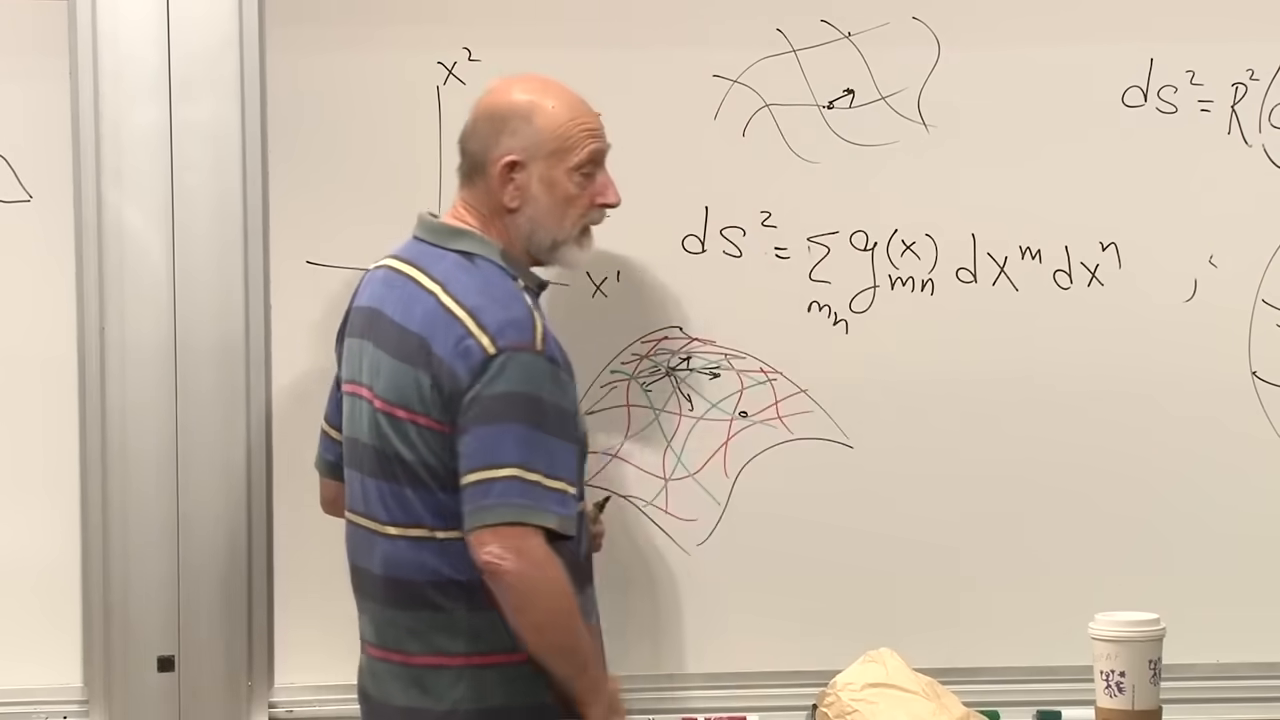
\includegraphics[width=\linewidth]{lecture_01_figure_04.png}
\caption{Réseau d’espace-temps linéaire pour des coordonnées en mouvement uniforme.}
\par\smallskip
\textit{Cadre du cours : 00:19:45.}
\end{figure}

Pour la transformation accélérée, une ligne où \(z'\) est constant vérifie
\begin{equation}
 z=z'+\frac12gt^2.
\end{equation}
C’est une parabole couchée. Si l’on prolonge le mouvement vers le passé, l’ascenseur descend en ralentissant, fait demi-tour, puis accélère vers le haut. Chaque ligne voisine où \(z'\) est constant est la même parabole, décalée horizontalement.

\begin{figure}[H]
\centering
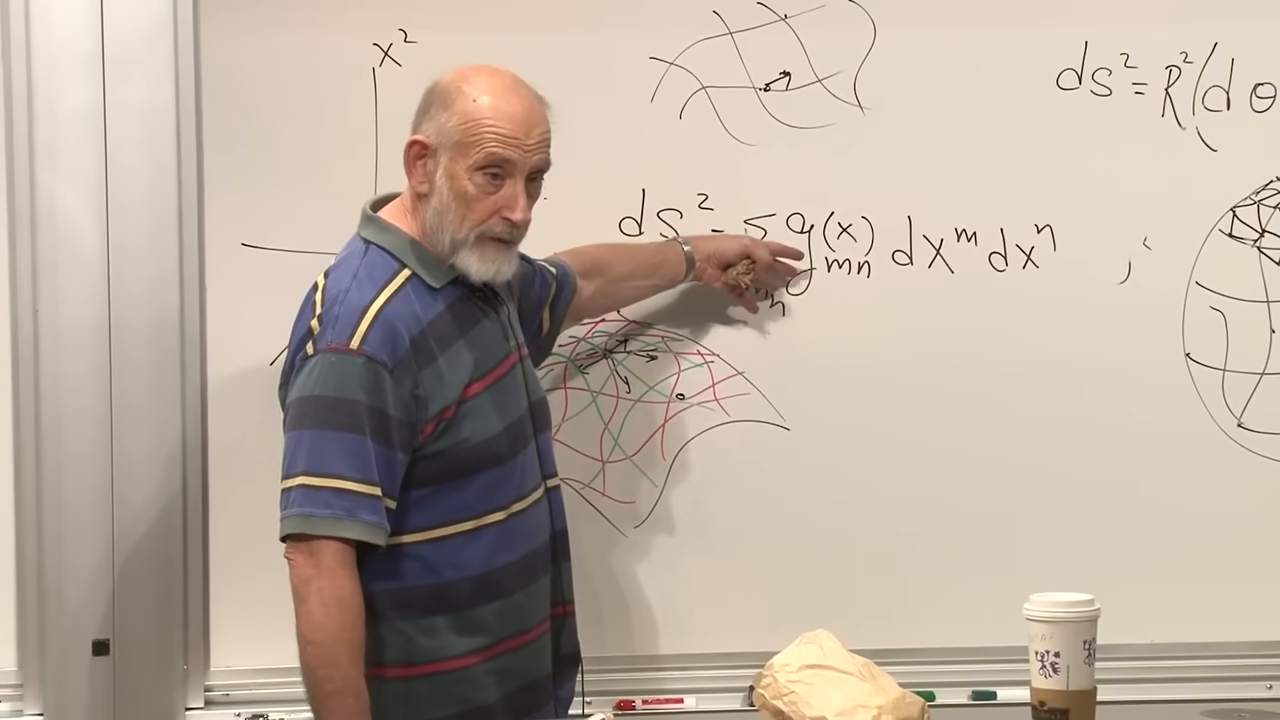
\includegraphics[width=\linewidth]{lecture_01_figure_05.png}
\caption{Courbes où \(z'\) est constant pour le système de coordonnées uniformément accéléré.}
\par\smallskip
\textit{Cadre du cours : 00:22:25.}
\end{figure}

Voici un premier indice géométrique. La relativité restreinte utilise des transformations de Lorentz linéaires, qui transforment les droites de l’espace-temps en droites de l’espace-temps. Pour représenter l’accélération et, par conséquent, imiter la gravitation, il faut des transformations curvilignes des coordonnées de l’espace-temps.

Einstein s’est servi de ce point apparemment modeste pour répondre à une question qui ne l’était pas du tout : la gravitation affecte-t-elle la lumière ? À \(t=0\), supposons que les référentiels de l’ascenseur et du sol soient momentanément au repos l’un par rapport à l’autre, puis envoyons un rayon lumineux horizontal à travers l’ascenseur. Dans le référentiel non accéléré,
\begin{equation}
 x=ct,\qquad z=0.
\end{equation}
En utilisant \(z=z'+\tfrac12gt^2\), ce même rayon, exprimé dans les coordonnées de l’ascenseur, vérifie
\begin{equation}
 z'=-\frac12gt^2
    =-\frac{g}{2c^2}x^2.
\label{eq:accelerated-light}
\end{equation}
Le rayon lumineux est rectiligne dans le référentiel inertiel et courbe dans le référentiel accéléré. Si l’accélération et la gravitation sont localement équivalentes, un champ gravitationnel doit dévier la lumière. Cet argument établit cet effet avant même qu’une équation de champ pour la gravitation ait été écrite.

\begin{figure}[H]
\centering
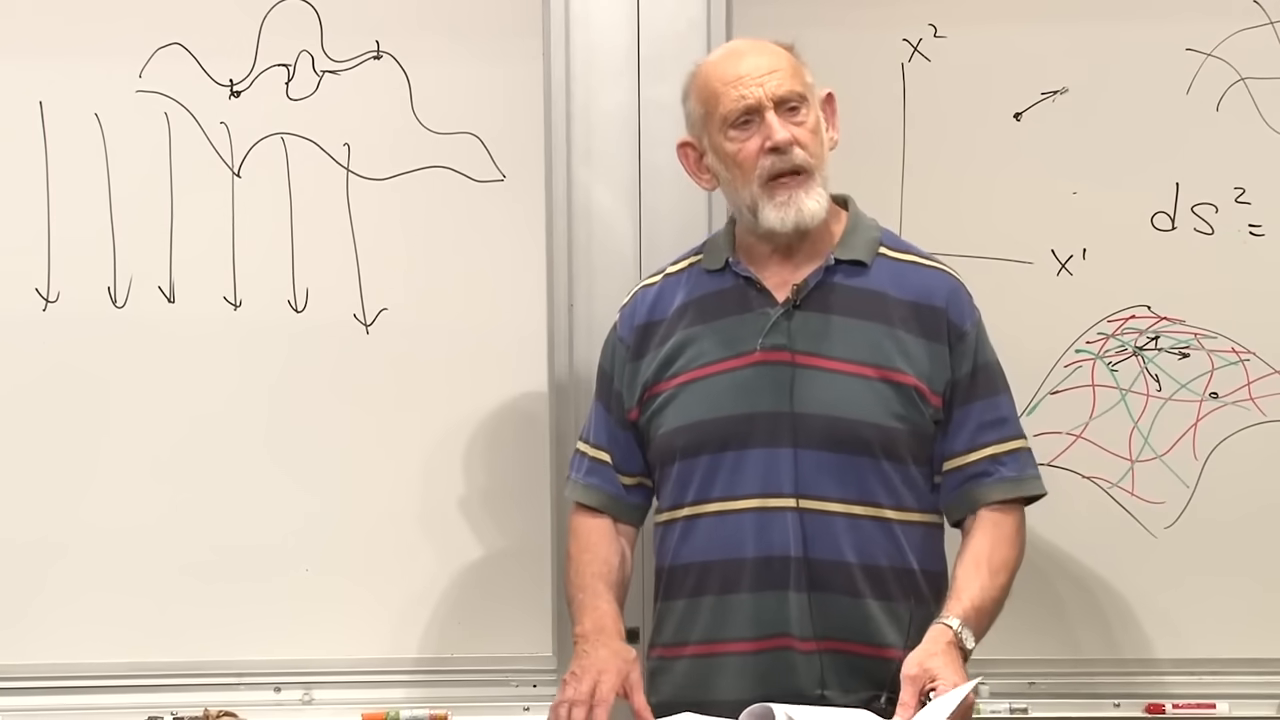
\includegraphics[width=\linewidth]{lecture_01_figure_06.png}
\caption{Rayon lumineux horizontal et trajectoire courbe dans le référentiel accéléré.}
\par\smallskip
\textit{Cadre du cours : 00:28:10.}
\end{figure}

\section{Ce qu’une transformation ne peut pas éliminer}

Un référentiel accéléré peut faire apparaître un champ gravitationnel uniforme. Cela ne signifie pas que tout champ gravitationnel soit un artefact de coordonnées. Le champ d’une étoile est dirigé radialement vers l’intérieur. Un petit laboratoire en chute libre près d’un point peut éliminer l’accélération locale, mais la même transformation ne peut éliminer le champ en tous les points autour de l’étoile.

\begin{figure}[H]
\centering
\includegraphics[width=\linewidth]{lecture_01_figure_07.png}
\caption{Champ radial et corps étendu en chute, utilisés pour mettre en évidence l’accélération de marée.}
\par\smallskip
\textit{Cadre du cours : 00:32:50.}
\end{figure}

L’obstacle est la force de marée. Imaginons une personne de deux mille miles de long qui tombe les pieds en avant. Ses pieds, plus proches de la source, accélèrent davantage que sa tête, ce qui l’étire. Tournée sur le côté, elle est comprimée, car les composantes des directions vers l’intérieur, de part et d’autre de son corps, sont orientées l’une vers l’autre. En termes newtoniens, des points voisins séparés par \(\xi^j\) acquièrent une accélération relative
\begin{equation}
 \delta a^i \simeq \partial_j g^i\,\xi^j.
\label{eq:newtonian-tide}
\end{equation}
On peut éliminer une accélération de coordonnées. En revanche, on ne peut éliminer l’accélération relative entre les points d’un corps étendu en chute libre.

\begin{classroomqa}
\audiencequestion{Des moteurs-fusées différents à la tête et aux pieds pourraient-ils simuler l’étirement et donc un champ de marée ?}
\lecturerresponse{Des moteurs appliqués peuvent certainement soumettre un corps à des contraintes, mais il s’agit alors d’une force réelle, non gravitationnelle, qui agit différemment sur ses parties. Un simple changement de coordonnées ne peut créer une accélération relative invariante entre des particules voisines en chute libre. Le diagnostic porte sur la chute libre sans force appliquée, et non sur un corps propulsé par des fusées distinctes.
\lecturetimestamp{00:36:51}}
\end{classroomqa}

Des coordonnées courbes peuvent néanmoins donner aux champs fictifs une apparence assez complexe. Un référentiel peut accélérer verticalement tout en oscillant horizontalement, ce qui produit un champ apparent dépendant du temps et comportant les deux composantes. Les coordonnées polaires ordinaires fournissent elles aussi un exemple instructif. Une particule libre qui se déplace en ligne droite dans les coordonnées cartésiennes voit d’abord \(r(t)\) diminuer, atteindre un rayon minimal, puis \(r(t)\) augmenter. Quelqu’un qui ne connaît que \(r(t)\) et \(\theta(t)\) pourrait en déduire l’existence d’une force répulsive dirigée vers l’extérieur. Dans les variantes tournantes de ces coordonnées apparaissent des termes centrifuges et de Coriolis. Ils sont proportionnels à la masse et ressemblent donc à des effets gravitationnels, mais ils ne produisent aucune déformation de marée invariante sur un corps en chute libre.

\begin{classroomqa}
\audiencequestion{Que se passe-t-il si le mouvement est décrit en coordonnées angulaires ou polaires ?}
\lecturerresponse{La description non linéaire en coordonnées donne l’impression qu’une trajectoire libre rectiligne est repoussée à partir de \(r=0\). Cette force centrifuge effective est une force de coordonnées. Le retour à un référentiel inertiel cartésien la fait disparaître et révèle qu’il n’y a aucune déformation de marée.
\lecturetimestamp{00:37:56}}
\end{classroomqa}

\begin{figure}[H]
\centering
\includegraphics[width=\linewidth]{lecture_01_figure_08.png}
\caption{Description en coordonnées polaires d’une trajectoire rectiligne, avec \(r(t)\) et \(\theta(t)\) indiqués au tableau.}
\par\smallskip
\textit{Cadre du cours : 00:40:20.}
\end{figure}

\begin{classroomqa}
\audiencequestion{Plusieurs corps gravitationnels peuvent-ils se compenser et ne laisser aucune force de marée ?}
\lecturerresponse{Les forces peuvent se compenser en un point donné, mais l’annulation de la valeur du champ n’annule généralement pas ses dérivées spatiales. Au voisinage de chaque source, les trajectoires voisines acquièrent toujours des accélérations différentes. Pour qu’il n’y ait véritablement pas de courbure, le diagnostic de marée doit être nul dans toute la région, et pas seulement la force nette en un point. \lecturetimestamp{00:42:16}}
\end{classroomqa}

\begin{classroomqa}
\audiencequestion{Comment mesure-t-on une force de marée en pratique ?}
\lecturerresponse{On laisse tomber en chute libre un objet étendu, par exemple un cristal, et l’on recherche les contraintes et déformations qui l’étirent dans une direction et le compriment dans une autre. Ces déformations sont mesurables et ne disparaissent pas quand on change les coordonnées. \lecturetimestamp{00:44:38}}
\end{classroomqa}

\begin{classroomqa}
\audiencequestion{Une personne de deux mille miles de long assise sur un manège ressentirait-elle un effet de marée radial ?}
\lecturerresponse{Une personne attachée au manège ressent des forces de soutien et peut effectivement avoir mal à la tête. Il faut plutôt que l’objet d’épreuve soit en chute libre. Sa trajectoire paraît complexe dans les coordonnées tournantes, mais reste une trajectoire rectiligne sans contrainte dans le référentiel inertiel ; la force de marée invariante est donc nulle.
\lecturetimestamp{00:45:07}}
\end{classroomqa}

\begin{classroomqa}
\audiencequestion{Peut-on incliner le corps en chute de façon que l’étirement et la compression se compensent ?}
\lecturerresponse{Aucune orientation unique ne supprime la déformation dans son ensemble. Le champ radial étire le corps selon une direction principale et le comprime selon les directions transversales. Un corps d’extension finie dans toutes les directions subit la déformation complète. \lecturetimestamp{00:47:10}}
\end{classroomqa}

\begin{figure}[H]
\centering
\includegraphics[width=\linewidth]{lecture_01_figure_09.png}
\caption{Étirement radial et compression transversale représentés ensemble pour un corps étendu en chute libre.}
\par\smallskip
\textit{Cadre du cours : 00:47:55.}
\end{figure}

\begin{classroomqa}
\audiencequestion{Les forces de marée signifient-elles que le principe d’équivalence échoue ?}
\lecturerresponse{Elles déterminent la précision avec laquelle il faut énoncer ce principe. Dans un système assez petit pour que le champ gravitationnel varie de façon négligeable à travers lui, un référentiel en chute libre permet d’éliminer la gravitation avec la précision voulue. La variation résiduelle dans un système plus étendu constitue le champ de marée. \lecturetimestamp{00:48:08}}
\end{classroomqa}

\section{De la géométrie de Minkowski à une métrique locale}

Mettons momentanément la gravitation de côté. Minkowski avait déjà montré que l’espace-temps possède une géométrie locale invariante. En une dimension spatiale, avec \(c=1\),
\begin{equation}
 d\tau^2=dt^2-dx^2.
\label{eq:minkowski-proper-time}
\end{equation}
On peut aussi définir \(ds^2=dx^2-dt^2=-d\tau^2\). La différence tient à une convention de signature, et non à une différence physique.

\begin{classroomqa}
\audiencequestion{Où intervient la vitesse de la lumière si on ne la pose pas égale à un ?}
\lecturerresponse{Si \(t\) est mesuré en unités de temps et \(x\) en unités de longueur, une forme commode est
\(d\tau^2=dt^2-dx^2/c^2\). De manière équivalente, on multiplie par \(c^2\) et l’on utilise
\(c^2d\tau^2=c^2dt^2-dx^2\). Le choix de \(ct\) ou de \(x/c\) comme coordonnée absorbe le facteur de conversion. \lecturetimestamp{00:51:02}}
\end{classroomqa}

\begin{figure}[H]
\centering
\includegraphics[width=\linewidth]{lecture_01_figure_10.png}
\caption{Intervalle de temps propre, qui établit le lien géométrique entre relativité restreinte et relativité générale.}
\par\smallskip
\textit{Cadre du cours : 00:51:10.}
\end{figure}

Einstein a reconnu que la question de savoir si un champ gravitationnel peut être éliminé ressemble à un problème étudié par Gauss pour les surfaces et par Riemann en dimensions quelconques : étant donnée une loi locale de distance, comment déterminer si la géométrie est véritablement courbe ?

En coordonnées cartésiennes euclidiennes, le théorème de Pythagore donne
\begin{equation}
 ds^2=(dx^1)^2+(dx^2)^2+\cdots
     =\delta_{mn}\,dx^m dx^n.
\label{eq:euclidean-line-element}
\end{equation}
La plage des indices correspond à la dimension de l’espace. La notation ne change pas selon qu’il y a deux, trois ou vingt-six coordonnées.

\begin{figure}[H]
\centering
\includegraphics[width=\linewidth]{lecture_01_figure_11.png}
\caption{Élément de longueur euclidien écrit comme somme de carrés des accroissements de coordonnées.}
\par\smallskip
\textit{Cadre du cours : 00:55:00.}
\end{figure}

Plaçons des coordonnées arbitraires \(x^m\) sur une surface quelconque. La distance entre deux points voisins est donnée par la forme quadratique
\begin{equation}
 ds^2=g_{mn}(x)\,dx^m dx^n.
\label{eq:general-line-element}
\end{equation}
Les fonctions \(g_{mn}(x)\) sont les composantes du tenseur métrique. La même formule s’applique aussi à une surface plane décrite en coordonnées curvilignes ; des composantes métriques non constantes ne prouvent pas, à elles seules, l’existence d’une courbure intrinsèque.

\begin{figure}[H]
\centering
\includegraphics[width=\linewidth]{lecture_01_figure_12.png}
\caption{Forme quadratique métrique générale représentée à côté d’un réseau de coordonnées courbes.}
\par\smallskip
\textit{Cadre du cours : 00:58:20.}
\end{figure}

Pour une sphère de rayon \(R\), lorsque \(\theta\) est mesuré à partir d’un pôle,
\begin{equation}
 ds^2=R^2\left(d\theta^2+\sin^2\theta\,d\phi^2\right).
\label{eq:sphere-polar}
\end{equation}
Un même accroissement de longitude couvre une grande distance près de l’équateur et une petite distance près d’un pôle ; cette dépendance à la position est précisément ce que traduit le coefficient.

\begin{classroomqa}
\audiencequestion{La latitude ordinaire étant mesurée depuis l’équateur, le coefficient ne devrait-il pas être un cosinus plutôt qu’un sinus ?}
\lecturerresponse{Oui. Si \(\lambda\) désigne la latitude mesurée depuis l’équateur, alors
\(ds^2=R^2(d\lambda^2+\cos^2\lambda\,d\phi^2)\).
L’équation \eqref{eq:sphere-polar} utilise l’angle polaire
\(\theta=\pi/2-\lambda\), mesuré depuis le pôle Nord.
\lecturetimestamp{01:01:03}}
\end{classroomqa}

\begin{figure}[H]
\centering
\includegraphics[width=\linewidth]{lecture_01_figure_13.png}
\caption{Métrique de la sphère et géométrie latitude--longitude qui déterminent son coefficient dépendant de la position.}
\par\smallskip
\textit{Cadre du cours : 01:00:30.}
\end{figure}

Des coordonnées plus générales peuvent introduire des termes croisés \(d\theta\,d\phi\), mais la distance locale reste une forme quadratique des différentielles. Les termes cubiques ou linéaires n’ont pas leur place dans un élément de longueur riemannien.

\section{Distance locale et courbure intrinsèque}

\begin{classroomqa}
\audiencequestion{La formule de la métrique donne-t-elle aussi la distance entre deux points très éloignés ?}
\lecturerresponse{Pas par simple substitution. Elle donne la distance entre des points voisins. Pour une distance macroscopique, il faut un chemin et une intégrale de \(ds\) ; si l’on entend par distance la longueur du plus court chemin, il faut également trouver ce chemin à partir de la géométrie. Plusieurs chemins localement minimaux peuvent même relier les mêmes extrémités. \lecturetimestamp{01:02:30}}
\end{classroomqa}

Sur une surface accidentée, imaginons deux piquets placés en des points éloignés et une corde tendue entre eux. La corde peut contourner une colline d’un côté ou de l’autre, et déplacer une colline change le trajet qui minimise la distance. La distance globale dépend de la géométrie entre les deux points. La distance locale est plus simple : la métrique fournit une petite règle en chaque point, et la géométrie se construit à partir de ces règles infinitésimales.

\begin{figure}[H]
\centering
\includegraphics[width=\linewidth]{lecture_01_figure_14.png}
\caption{Problème de la distance globale : un trajet tendu doit traverser la surface entre ses extrémités.}
\par\smallskip
\textit{Cadre du cours : 01:04:00.}
\end{figure}

Si l’on peut poser les éléments locaux sur un plan sans les étirer ni les déchirer, la géométrie intrinsèque est plate. Des éléments ayant les longueurs d’une sphère triangulée ne peuvent pas tous être posés à plat tout en conservant leurs arêtes. La métrique permet donc de poser un problème précis : étant donné \(g_{mn}(x)\), peut-on déterminer si ses éléments infinitésimaux s’assemblent en un espace plat ?

\begin{figure}[H]
\centering
\includegraphics[width=\linewidth]{lecture_01_figure_15.png}
\caption{La métrique et la carte locale de coordonnées, interprétées comme les éléments infinitésimaux qui composent la géométrie.}
\par\smallskip
\textit{Cadre du cours : 01:05:20.}
\end{figure}

\begin{classroomqa}
\audiencequestion{Peut-on diagnostiquer la courbure en mesurant le rapport entre la circonférence et le diamètre ?}
\lecturerresponse{Oui, c’est un test utile en deux dimensions. Sur une surface courbe, le rapport peut différer de \(\pi\). Toutefois, pour un cercle infinitésimal, l’écart n’apparaît qu’à un ordre supérieur, et cette méthode ne se généralise pas aussi simplement qu’un tenseur de courbure.
\lecturetimestamp{01:07:26}}
\end{classroomqa}

Une région est plate s’il existe un système de coordonnées dans lequel
\begin{equation}
 g_{mn}=\delta_{mn},
\qquad
 ds^2=\delta_{mn}\,dx^m dx^n
\label{eq:flat-metric}
\end{equation}
dans toute cette région. Une métrique \(g_{mn}(x)\) compliquée peut donc décrire soit un espace courbe, soit simplement des coordonnées courbes dans un espace plat. Il s’agit de savoir si une transformation de coordonnées peut éliminer toutes les complications.

\begin{figure}[H]
\centering
\includegraphics[width=\linewidth]{lecture_01_figure_16.png}
\caption{Le problème métrique posé sur une carte locale de coordonnées : peut-on transformer sa forme curviligne pour obtenir la forme plate ?}
\par\smallskip
\textit{Cadre du cours : 01:07:15.}
\end{figure}

\begin{classroomqa}
\audiencequestion{L’élément de longueur sphérique suppose-t-il que chaque petit intervalle soit plat, même si la sphère ne l’est pas ?}
\lecturerresponse{Au premier ordre, toute surface régulière est approximée en un point par son plan tangent. La courbure se manifeste dans la façon dont les approximations tangentes voisines cessent de s’ajuster les unes aux autres, ou dans les variations d’ordre supérieur à travers une carte finie. Le comportement euclidien local et la courbure globale sont donc compatibles. \lecturetimestamp{01:10:01}}
\end{classroomqa}

\begin{classroomqa}
\audiencequestion{La métrique doit-elle être continue, et que se passe-t-il au niveau d’un pli ou d’un creux ?}
\lecturerresponse{Cette discussion suppose que les cartes de coordonnées et la métrique sont suffisamment régulières pour que les dérivées requises existent. Une feuille pliée sans être étirée conserve les mêmes distances intrinsèques de part et d’autre du pli ; son apparence spectaculaire est extrinsèque. Une géométrie véritablement singulière ou non régulière demande des précautions particulières et sort du cadre régulier adopté ici. \lecturetimestamp{01:11:25}}
\end{classroomqa}

Cette distinction relève de la géométrie intrinsèque. Plier une feuille dans l’espace tridimensionnel modifie son plongement, mais pas les distances mesurées sur la feuille. Une créature confinée à la feuille, incapable de regarder l’espace dans lequel elle est plongée, peut tout de même mesurer sa géométrie intrinsèque.

\begin{figure}[H]
\centering
\includegraphics[width=\linewidth]{lecture_01_figure_17.png}
\caption{Feuille pliée permettant de distinguer la distance intrinsèque de l’apparence extrinsèque.}
\par\smallskip
\textit{Cadre du cours : 01:13:00.}
\end{figure}

\begin{classroomqa}
\audiencequestion{Pourquoi ne pas simplement diagonaliser la métrique ?}
\lecturerresponse{En un point donné, un choix approprié de coordonnées permet de diagonaliser la métrique et de la ramener à la forme locale plate. L’obstacle consiste à y parvenir dans toute une région avec un seul système de coordonnées. On ne peut pas détecter la courbure en examinant un point isolément.
\lecturetimestamp{01:13:48}}
\end{classroomqa}

\begin{figure}[H]
\centering
\includegraphics[width=\linewidth]{lecture_01_figure_18.png}
\caption{La métrique cartésienne plate \(\delta_{mn}\) écrite sous la forme quadratique locale générale.}
\par\smallskip
\textit{Cadre du cours : 01:16:00.}
\end{figure}

L’analogie avec la gravitation est maintenant exacte et non plus seulement suggestive. Une force de coordonnées peut être éliminée, tout comme on peut éliminer une description curviligne d’un espace plat. En relativité générale, l’accélération de marée se mesure par la courbure. Dans la notation qui sera introduite plus loin, des lignes d’univers voisines en chute libre vérifient l’équation de déviation géodésique
\begin{equation}
 \frac{D^2\xi^\mu}{D\tau^2}
 =-R^\mu{}_{\nu\rho\sigma}
   u^\nu\xi^\rho u^\sigma.
\label{eq:geodesic-deviation-preview}
\end{equation}
Une courbure nulle signifie qu’il n’y a pas de champ de marée invariant ; une courbure non nulle signifie qu’aucun choix de coordonnées ne peut éliminer la gravitation dans toute la région.

\section{Deux systèmes de coordonnées et un vecteur}

Pour déterminer si une métrique peut être transformée en \(\delta_{mn}\), il faut d’abord savoir comment se transforment les objets géométriques. Soient \(x^m\) et \(y^m\) deux systèmes de coordonnées réguliers définis sur la même région :
\begin{equation}
 x^m=x^m(y),\qquad y^m=y^m(x).
\label{eq:mutual-coordinate-maps}
\end{equation}
Les symboles \(x\) et \(y\) désignent des systèmes de coordonnées complets, et non deux directions spatiales particulières.

\begin{figure}[H]
\centering
\includegraphics[width=\linewidth]{lecture_01_figure_19.png}
\caption{Applications coordonnées réciproques \(x^m(y)\) et \(y^m(x)\).}
\par\smallskip
\textit{Cadre du cours : 01:20:35.}
\end{figure}

Pour des points voisins, la règle de dérivation en chaîne donne
\begin{equation}
 dy^m=\frac{\partial y^m}{\partial x^p}\,dx^p.
\label{eq:differential-transform}
\end{equation}
L’indice répété \(p\) indique une sommation. Le déplacement est un seul vecteur géométrique ; \(dx^p\) et \(dy^m\) en sont les composantes dans deux systèmes de coordonnées.

\begin{figure}[H]
\centering
\includegraphics[width=\linewidth]{lecture_01_figure_20.png}
\caption{Transformation différentielle de coordonnées obtenue par la règle de dérivation en chaîne.}
\par\smallskip
\textit{Cadre du cours : 01:22:30.}
\end{figure}

\begin{classroomqa}
\audiencequestion{Sur une grille curviligne, que représentent les lignes de coordonnées ?}
\lecturerresponse{En deux dimensions, on obtient une ligne en maintenant une coordonnée fixe tout en faisant varier l’autre. En dimensions supérieures, les ensembles où une coordonnée est constante sont des hypersurfaces. Leurs intersections locales définissent les directions de coordonnées utilisées pour décomposer les vecteurs en composantes. \lecturetimestamp{01:25:20}}
\end{classroomqa}

Un vecteur contravariant est défini par la même loi de transformation qu’un déplacement de coordonnées :
\begin{equation}
 (V')^m(y)
 =\frac{\partial y^m}{\partial x^p}\,V^p(x).
\label{eq:contravariant-vector}
\end{equation}
La vitesse le long d’une surface en est un exemple. Le vecteur ne change pas lorsque les coordonnées changent ; ses composantes, elles, changent.

\begin{figure}[H]
\centering
\includegraphics[width=\linewidth]{lecture_01_figure_21.png}
\caption{Loi de transformation d’un vecteur contravariant encadrée.}
\par\smallskip
\textit{Cadre du cours : 01:29:30.}
\end{figure}

La convention de sommation d’Einstein omet le signe de sommation lorsqu’un indice apparaît une fois en haut et une fois en bas. Cette convention facilite l’écriture des formules, mais, surtout, rend visible la structure des contractions.

\begin{classroomqa}
\audiencequestion{Fait-on des hypothèses particulières sur les systèmes de coordonnées admissibles ?}
\lecturerresponse{On suppose seulement que les deux systèmes sont liés par des fonctions et suffisamment réguliers pour que les dérivées indiquées et l’application réciproque existent dans la région considérée. On ne suppose ni linéarité ni orthogonalité. \lecturetimestamp{01:28:12}}
\end{classroomqa}

\section{Covecteurs et règle de dérivation en chaîne}

Soit \(S(x)\) un scalaire : il possède en chaque point une valeur bien définie, indépendante des étiquettes de coordonnées. La température et un champ scalaire en sont des exemples. Les composantes de son gradient sont
\begin{equation}
 W_p=\frac{\partial S}{\partial x^p}.
\label{eq:gradient-covector}
\end{equation}

\begin{figure}[H]
\centering
\includegraphics[width=\linewidth]{lecture_01_figure_22.png}
\caption{Gradient d’un scalaire présenté à côté de la loi de transformation contravariante.}
\par\smallskip
\textit{Cadre du cours : 01:31:40.}
\end{figure}

En appliquant la règle de dérivation en chaîne dans les coordonnées \(y\),
\begin{equation}
 W'_m
 =\frac{\partial S}{\partial y^m}
 =\frac{\partial x^p}{\partial y^m}
  \frac{\partial S}{\partial x^p}
 =\frac{\partial x^p}{\partial y^m}\,W_p.
\label{eq:covariant-vector}
\end{equation}
C’est la loi de transformation d’un vecteur covariant, ou covecteur. La jacobienne est l’inverse de celle de
\eqref{eq:contravariant-vector} ; les indices inférieurs et supérieurs encodent donc des comportements de transformation différents.

\begin{figure}[H]
\centering
\includegraphics[width=\linewidth]{lecture_01_figure_23.png}
\caption{Lois de transformation contravariante et covariante présentées côte à côte.}
\par\smallskip
\textit{Cadre du cours : 01:34:40.}
\end{figure}

\begin{classroomqa}
\audiencequestion{Quel est le lien entre les vecteurs covariants et contravariants ?}
\lecturerresponse{À ce stade, ils sont définis comme des objets de types différents : les déplacements et les vitesses se transforment d’une manière, les gradients de la manière inverse. La métrique fournira plus tard une application bijective qui abaisse ou relève un indice. Il ne faut pas présupposer ce lien avant d’avoir introduit la métrique. \lecturetimestamp{01:37:43}}
\end{classroomqa}

\begin{classroomqa}
\audiencequestion{La baisse d’un indice a-t-elle précédemment changé le signe de la composante temporelle ?}
\lecturerresponse{Ce signe venait de la métrique lorentzienne. Pour l’instant, la dérivation se fait d’abord en géométrie euclidienne ordinaire. La montée ou la baisse d’un indice fait toujours intervenir la métrique appropriée ; un changement de signe de la composante temporelle n’apparaît que lorsque cette métrique est de signature lorentzienne.
\lecturetimestamp{01:38:29}}
\end{classroomqa}

\begin{classroomqa}
\audiencequestion{Faut-il déjà considérer les deux lois de transformation comme deux descriptions en composantes d’un même vecteur ?}
\lecturerresponse{Pas encore. Une fois la métrique disponible, un vecteur contravariant \(V^m\) peut être converti en un covecteur \(V_m=g_{mn}V^n\). Tant que cette application n’a pas été établie, les objets à indices supérieurs et inférieurs sont logiquement distincts. \lecturetimestamp{01:39:00}}
\end{classroomqa}

Ces formules sont indépendantes de la dimension. La plage des indices change, mais pas les lois de transformation.

\section{Tenseurs à plusieurs indices}

Considérons deux vecteurs contravariants \(V^m\) et \(U^n\). Leur produit
\begin{equation}
 T^{mn}=V^mU^n
\label{eq:rank-two-product}
\end{equation}
est un tenseur contravariant de rang deux. En trois dimensions, il possède neuf composantes ; en quatre dimensions, il en possède seize. L’ordre des indices importe, sauf si une symétrie particulière est spécifiée : \(T^{mn}\) n’est pas nécessairement égal à \(T^{nm}\).

\begin{figure}[H]
\centering
\includegraphics[width=\linewidth]{lecture_01_figure_24.png}
\caption{Un tenseur de rang deux construit comme le produit de deux vecteurs contravariants.}
\par\smallskip
\textit{Image de la leçon : 01:43:40.}
\end{figure}

Chaque indice supérieur apporte un facteur de jacobienne directe :
\begin{equation}
 (T')^{mn}
 =\frac{\partial y^m}{\partial x^p}
  \frac{\partial y^n}{\partial x^q}
  T^{pq}.
\label{eq:rank-two-contravariant}
\end{equation}
La construction par produit motive cette règle, mais c’est la loi de transformation qui définit un tenseur. Un tenseur contravariant de rang trois acquiert trois facteurs de jacobienne de ce type.

\begin{figure}[H]
\centering
\includegraphics[width=\linewidth]{lecture_01_figure_25.png}
\caption{Les deux facteurs de jacobienne dans la transformation de \(T^{mn}\).}
\par\smallskip
\textit{Image de la leçon : 01:44:20.}
\end{figure}

De même, chaque indice inférieur apporte un facteur de jacobienne inverse :
\begin{equation}
 T'_{mn}
 =\frac{\partial x^p}{\partial y^m}
  \frac{\partial x^q}{\partial y^n}
  T_{pq}.
\label{eq:rank-two-covariant}
\end{equation}
Un tenseur mixte comporte un facteur de chaque type.

\begin{figure}[H]
\centering
\includegraphics[width=\linewidth]{lecture_01_figure_26.png}
\caption{La loi de transformation complète d’un tenseur à deux indices covariants.}
\par\smallskip
\textit{Image de la leçon : 01:47:30.}
\end{figure}

Le même mécanisme de transformation s’applique maintenant à la métrique. Puisque l’intervalle est un scalaire, il doit avoir la même valeur dans les deux systèmes de coordonnées :
\begin{align}
 ds^2
 &=g_{mn}(x)\,dx^m dx^n,\\
 dx^m
 &=\frac{\partial x^m}{\partial y^p}\,dy^p.
\end{align}
La substitution complète la ligne laissée inachevée au tableau :
\begin{equation}
 g'_{pq}(y)
 =\frac{\partial x^m}{\partial y^p}
  \frac{\partial x^n}{\partial y^q}
  g_{mn}(x(y)).
\label{eq:l1-metric-transformation}
\end{equation}
Ainsi, \(g_{mn}\) est un tenseur covariant de rang deux.

\begin{figure}[H]
\centering
\includegraphics[width=\linewidth]{lecture_01_figure_27.png}
\caption{La transformation de la métrique, amorcée à partir de l’invariance de l’élément de ligne à la fin de la leçon.}
\par\smallskip
\textit{Image de la leçon : 01:48:40.}
\end{figure}

La question physique posée au départ est désormais devenue une question mathématique. Étant donné \(g_{mn}(x)\), existe-t-il une transformation de coordonnées telle que \(g'_{mn}=\delta_{mn}\) dans toute la région ? Si oui, la complexité apparente n’est qu’une complexité due aux coordonnées. Sinon, l’obstacle est la courbure, et dans l’espace-temps cet obstacle constitue le contenu invariant de la gravité.